\documentclass[authoryear,preprint,12pt]{elsarticle}

\usepackage{amsmath,amssymb,amsfonts}
\usepackage{lmodern}
\usepackage{graphicx}
\usepackage{booktabs}
\usepackage{tabularx}
\usepackage{multirow}
\usepackage{lineno}
\usepackage{hyperref}
\usepackage{microtype}
\usepackage[margin=2.5cm]{geometry}

\journal{Environmental Research}

\begin{document}

\begin{frontmatter}

\title{Can Published Evidence Support National-Scale Inference on Metal Contamination in Bangladesh's Rivers? A Critical Systematic Review of Analytical Comparability, Spatial Representativeness, and Ecological Risk Assessment}

\author[inst1]{Author One\corref{cor1}}
\ead{author.one@university.edu}
\author[inst1,inst2]{Author Two}
\ead{author.two@institution.org}
\author[inst2]{Author Three}
\ead{author.three@research.org}

\cortext[cor1]{Corresponding author.}

\affiliation[inst1]{organization={Department of Environmental Science and Engineering},
            addressline={University Name}, 
            city={Dhaka},
            postcode={1000},
            country={Bangladesh}}

\affiliation[inst2]{organization={Institute of Water and Flood Management},
            addressline={Technical University}, 
            city={Dhaka},
            postcode={1205},
            country={Bangladesh}}

\begin{abstract}
Surface waters and bed sediments in the Ganges--Brahmaputra--Meghna (GBM) delta sustain the municipal water supplies, agriculture, and fisheries of over 170 million people. While dozens of independent investigations over the past two decades have documented heavy metal concentrations across individual river corridors, the published scientific literature remains fragmented across isolated case studies, conflicting analytical protocols, unharmonized regulatory criteria, and non-transparent reporting. Recent compilations have aggregated these records to present regional summaries of metal pollution, yet none have critically appraised whether the published evidence base is methodologically robust, analytically comparable, and geographically representative enough to support national-scale environmental governance. Here, we present a critical systematic review and evidence map following PRISMA 2020 and ROSES guidelines, synthesizing 28 peer-reviewed field investigations (2010--2025) comprising 557 verified analytical assays across 12 major river systems. We evaluate the evidence across eight methodological quality domains and five research questions ($RQ1$--$RQ5$). 

Our critical evidence appraisal reveals three profound systemic vulnerabilities in the published literature:
(1) \textbf{Analytical Incomparability and LOD Censoring ($RQ2$):} Flame atomic absorption spectrometry (Flame-AAS), deployed in 48.8\% of water assays, yields reported median concentrations two to six times higher than high-sensitivity graphite furnace AAS (GF-AAS) or inductively coupled plasma mass spectrometry (ICP-MS) (Pb: 0.110 vs.\ 0.0171~mg/L; Cr: 0.091 vs.\ 0.0461~mg/L; Ni: 0.120 vs.\ 0.0180~mg/L). This divergence is driven by high instrumental limits of detection (LOD: 0.010--0.050~mg/L) coupled with non-transparent reporting (46.4\% of studies omit LOD definitions or censor non-detects). Furthermore, only 58.7\% of surface water assays explicitly verified 0.45~$\mu\text{m}$ membrane filtration, confounding suspended mineral particulates with dissolved bioactive fractions. Certified reference material (CRM) verification was absent in 35.7\% of studies.
(2) \textbf{Geographical Representativeness and Spatial Deficits ($RQ3$):} Auditing 222 registered physical sampling stations demonstrates that 32.0\% ($n=71$) provide verifiable handheld GPS coordinates (Tier 1), 6.3\% ($n=14$) represent cartographically digitized centroids (Tier 2), and 61.7\% ($n=137$) remain unresolved descriptive gazetteer names (Tier 3). Snapping all 85 georeferenced stations to the HydroSHEDS HydroRIVERS topological reach network (2,224 reaches, 4,599.1~km; mean metric offset in UTM Zone 45N: 379.6~m, median: 262.1~m) reveals that pooling the entire literature corpus across both water and sediment covers only \textbf{21.8\% of major river corridor length (1,004.7~km)} at 25~km (6.8\% at 10~km), leaving \textbf{78.2\% of national major river corridors unmonitored} (expanding to 83.5\% unmonitored when evaluating surface-water heavy metals alone, 23 unique coordinates). Transboundary mainstems of the Padma, Jamuna, and Lower Meghna remain almost completely unmonitored.
(3) \textbf{Structural Fragility of Published Risk Indices ($RQ4$):} Critical appraisal reveals that published aquatic pollution assessments in Bangladesh have uncritically deployed composite risk indices without recognizing underlying structural artifacts. In surface waters, widely used formulations such as the Heavy Metal Pollution Index ($\mathrm{HPI}$) suffer from severe inverse statutory weighting damping that concentrates scores almost entirely on Cadmium and Lead, creating artificial panel invariance across disparate monitoring suites (as mathematically proven in companion regulatory work). In sediments, composite Hakanson potential ecological risk ($RI$) scores are overwhelmingly dominated ($>80\%$) by Cadmium due to arbitrary toxic-response factors ($T_r=30$) and uncalibrated continental crust baselines ($0.1\text{ mg/kg}$), lacking regional validation against benthic macroinvertebrate community health.

Finally, we audit compliance under the gazetted \textit{Environmental Conservation Rules 2023} (ECR 2023 Schedule 2), which lowered the statutory drinking threshold for Pb from 0.050 to 0.010~mg/L, surging raw-water drinking benchmark exceedance from 34.9\% to \textbf{85.6\%}. We outline an operational evidence-readiness framework ($RQ5$) and a reach-prioritized 15-sector blueprint for institutional surveillance by the Department of Environment (DoE) and Bangladesh Water Development Board (BWDB).
\end{abstract}

\begin{highlights}
\item First PRISMA 2020 \& ROSES critical evidence review of Bangladesh river heavy metals (2010--2025).
\item 8-Domain CEE appraisal across 28 studies (557 assays) reveals pervasive QA/QC gaps.
\item Flame-AAS inflates reported water medians 2$\times$--6$\times$ over GF-AAS/ICP-MS due to LOD censoring.
\item Auditing 222 physical stations reveals 61.7\% lack coordinates; literature covers only 21.8\% of river length.
\item Critical appraisal of risk indices reveals widespread failure to account for guideline damping and uncalibrated crustal baselines.
\item ECR 2023 statutory tightening elevates drinking benchmark exceedance from 34.9\% to 85.6\%.
\item Formulates an evidence-readiness monitoring framework and 15-reach transboundary deployment blueprint.
\end{highlights}

\begin{keyword}
Systematic Review \sep Evidence Map \sep PRISMA 2020 \sep ROSES \sep Heavy Metals \sep Analytical Comparability \sep Limit of Detection \sep Spatial Representativeness \sep ECR 2023 \sep Bengal Delta
\end{keyword}

\end{frontmatter}

\linenumbers

\section{Introduction}

The Bengal Delta, formed by the convergence of the Ganges, Brahmaputra, and Meghna (GBM) rivers, is one of the world's most densely populated and hydrologically active fluvio-deltaic systems \citep{Goodbred1999}. Over 170 million people in Bangladesh depend on its dense river network for agricultural irrigation (particularly dry-season \textit{boro} rice cultivation), artisanal freshwater capture fisheries, inland waterborne transportation, and raw water intake for metropolitan municipal water treatment plants \citep{BBS2022,Chowdhury2004}. However, rapid urban industrial expansion over the past three decades---centered around ready-made garment (RMG) textile wet processing, leather tanning, electroplating, chemical manufacturing, shipbreaking, and intensive agrochemical utilization---has introduced vast, untreated effluent loads directly into natural river corridors \citep{Islam2015,Bhuiyan2015,Hasan2024}.

Potentially toxic heavy metals and metalloids (e.g., As, Cd, Cr, Cu, Ni, Pb, Zn) represent an acute environmental threat due to their non-biodegradability, persistence across sediment-water interfaces, bioaccumulation through aquatic trophic webs, and severe systemic toxicity to human health and benthic ecosystems \citep{Hakanson1980,Jarup2003,Tchounwou2012}. In response to escalating public concern, dozens of independent academic research groups have collected water and bed sediment samples across various Bangladeshi river channels over the past fifteen years. 

Recently, several literature reviews have sought to synthesize this growing body of research. Notably, \citet{Pandit2025} compiled 55 publications (2001--2020) on heavy metals in Bangladesh river waters to summarize concentration ranges and health risk quotients. Similarly, a comprehensive multi-matrix synthesis in late 2025 reviewed 100 studies across soil, water, plants, and sediments from 2010 to 2024. While these narrative compilations provide useful bibliometric overviews and regional concentration summaries, they share a critical limitation: \textbf{they treat the published scientific literature as an unproblematic, homogeneous data repository}. By aggregating raw numerical concentrations reported across disparate papers without methodologically auditing analytical instrumentation, sample filtration protocols, detection limits, quality assurance verification, or spatial sampling designs, existing reviews risk amplifying systematic methodological artifacts into false national conclusions.

Crucially, five unresolved questions continue to paralyze both scientific consensus and environmental governance in Bangladesh:
\begin{enumerate}
    \item \textbf{RQ1 (Spatio-Temporal Evidence Landscape):} How has heavy metal research across Bangladesh's fluvial network evolved chronologically, geographically, and across environmental matrices (water vs.\ sediment)? Which specific river corridors dominate the literature, and which are systematically omitted?
    \item \textbf{RQ2 (Analytical Comparability and Detection Limit Censoring):} Are chemical concentrations reported across independent investigations directly comparable? To what degree do differences in analytical instrumentation (Flame-AAS vs.\ GF-AAS vs.\ ICP-MS), acid digestion protocols, phase filtration (0.45~$\mu\text{m}$ filtered dissolved vs.\ bulk total), and limit-of-detection (LOD) handling bias reported medians and compliance rates?
    \item \textbf{RQ3 (Spatial Representativeness and Coordinate Accuracy):} What is the true cartographic precision of reported sampling stations? When verified sampling points are integrated into topological stream network models (HydroSHEDS HydroRIVERS), what proportion of the national river network is empirically monitored versus unmonitored surveillance blind spots?
    \item \textbf{RQ4 (Methodological Robustness of Published Risk Indices):} How robust are the composite multi-metal pollution and ecological risk indices widely applied in Bangladesh literature---specifically the Heavy Metal Pollution Index ($\mathrm{HPI}$) for surface water and the Hakanson Potential Ecological Risk Index ($RI$) for sediments? Do reported indices reflect validated ambient ecological risks, or are they constrained by mathematical guideline weighting damping and uncalibrated continental crust baselines?
    \item \textbf{RQ5 (Evidence Readiness and National Surveillance Blueprint):} What technical criteria, QA/QC standards, statutory realignments (under Bangladesh's updated ECR 2023 Schedule 2), and geographical deployment priorities are required to transition from opportunistic academic publications to an institutionalized national river surveillance network?
\end{enumerate}

To answer these questions, this study provides the first comprehensive, PRISMA 2020- and ROSES-compliant systematic review and critical evidence map of heavy metal contamination in Bangladesh river systems (2010--2025). Rather than simply compiling another table of reported pollution values, we subject 28 peer-reviewed field investigations (557 validated analytical assays across 12 major river systems) to a rigorous eight-domain critical appraisal. We evaluate analytical comparability, appraise the structural limitations of published risk indices, map national hydrographic surveillance gaps across 2,224 river reaches, and deliver an evidence-readiness framework for future deltaic water governance.

\section{Materials and Methods}

\subsection{PRISMA 2020 and ROSES Systematic Search Protocol}
This systematic review and evidence synthesis was conducted in strict compliance with the Preferred Reporting Items for Systematic Reviews and Meta-Analyses (PRISMA 2020) statement \citep{Page2021} and the RepOrting standards for Systematic Evidence Syntheses (ROSES) in environmental research \citep{Haddaway2018ROSES,CEE2018}. A structured bibliographic search was executed across five academic literature databases: Web of Science Core Collection, Scopus, ScienceDirect, PubMed, and the Bangladesh National Scientific and Technical Documentation Centre (BANSDOC) for peer-reviewed studies published between January 1, 2010, and March 31, 2025.

The search strategy combined Boolean operators across three core conceptual facets:
\begin{quote}\small\raggedright
\texttt{("heavy metal*" OR "trace metal*" OR "trace element*" OR "toxic element*")} \\
\textbf{AND} \\
\texttt{("river water" OR "surface water" OR "river sediment" OR "bed sediment")} \\
\textbf{AND} \\
\texttt{("Bangladesh" OR "Bengal Delta" OR "Buriganga" OR "Karnaphuli" OR "Meghna" OR "Padma" OR "Jamuna" OR "Turag" OR "Surma" OR "Rupsa" OR "Korotoa")}
\end{quote}

\subsection{Study Eligibility Screening and Data Harmonization}
Search results were deduplicated and screened against five predefined eligibility criteria:
\begin{enumerate}
    \item \textbf{Target System:} Primary empirical field investigations collecting ambient water or bed sediment samples within natural flowing river corridors or estuarine channels strictly within Bangladesh. Studies on closed wastewater lagoons, agricultural soils, roadside dust, groundwater aquifers, or offshore marine shelf waters were excluded.
    \item \textbf{Target Analytes:} Quantitative numerical reporting for at least one target element: Lead (Pb), Chromium (Cr), Cadmium (Cd), Arsenic (As), Nickel (Ni), Copper (Cu), or Zinc (Zn).
    \item \textbf{Geographical Traceability:} Documented sampling locations identifiable via handheld GPS coordinates, detailed site maps, or unambiguous geographical landmarks.
    \item \textbf{Methodological Documentation:} Explicit reporting of sample collection protocols, digestion chemistry, analytical instrumentation, and quality control procedures.
    \item \textbf{Publication Type:} Original empirical research published in indexed, peer-reviewed scientific journals. Theses, conference abstracts, corporate reports, and review articles were excluded to avoid double-counting primary observations.
\end{enumerate}

Initial bibliographic queries retrieved 1,420 candidate records (Fig.~\ref{fig:prisma}). After automated and manual deduplication, 582 duplicate records were removed. The remaining 838 records were screened by title and abstract, excluding 764 records as off-topic (predominantly groundwater arsenic epidemiology, soil agrochemical surveys, or laboratory adsorption bench tests). Full texts of 74 articles were retrieved and scrutinized in detail. Forty-six articles were excluded due to irreconcilable methodological deficits: complete omission of sampling coordinates or maps ($n=18$), absence of analytical QA/QC or digestion descriptions ($n=15$), and aggregated regional averages lacking station-level granularity ($n=13$). Exactly 28 primary investigations met all inclusion criteria, yielding 557 harmonized analytical assays across 12 river systems.

\begin{figure}[htbp]
\centering
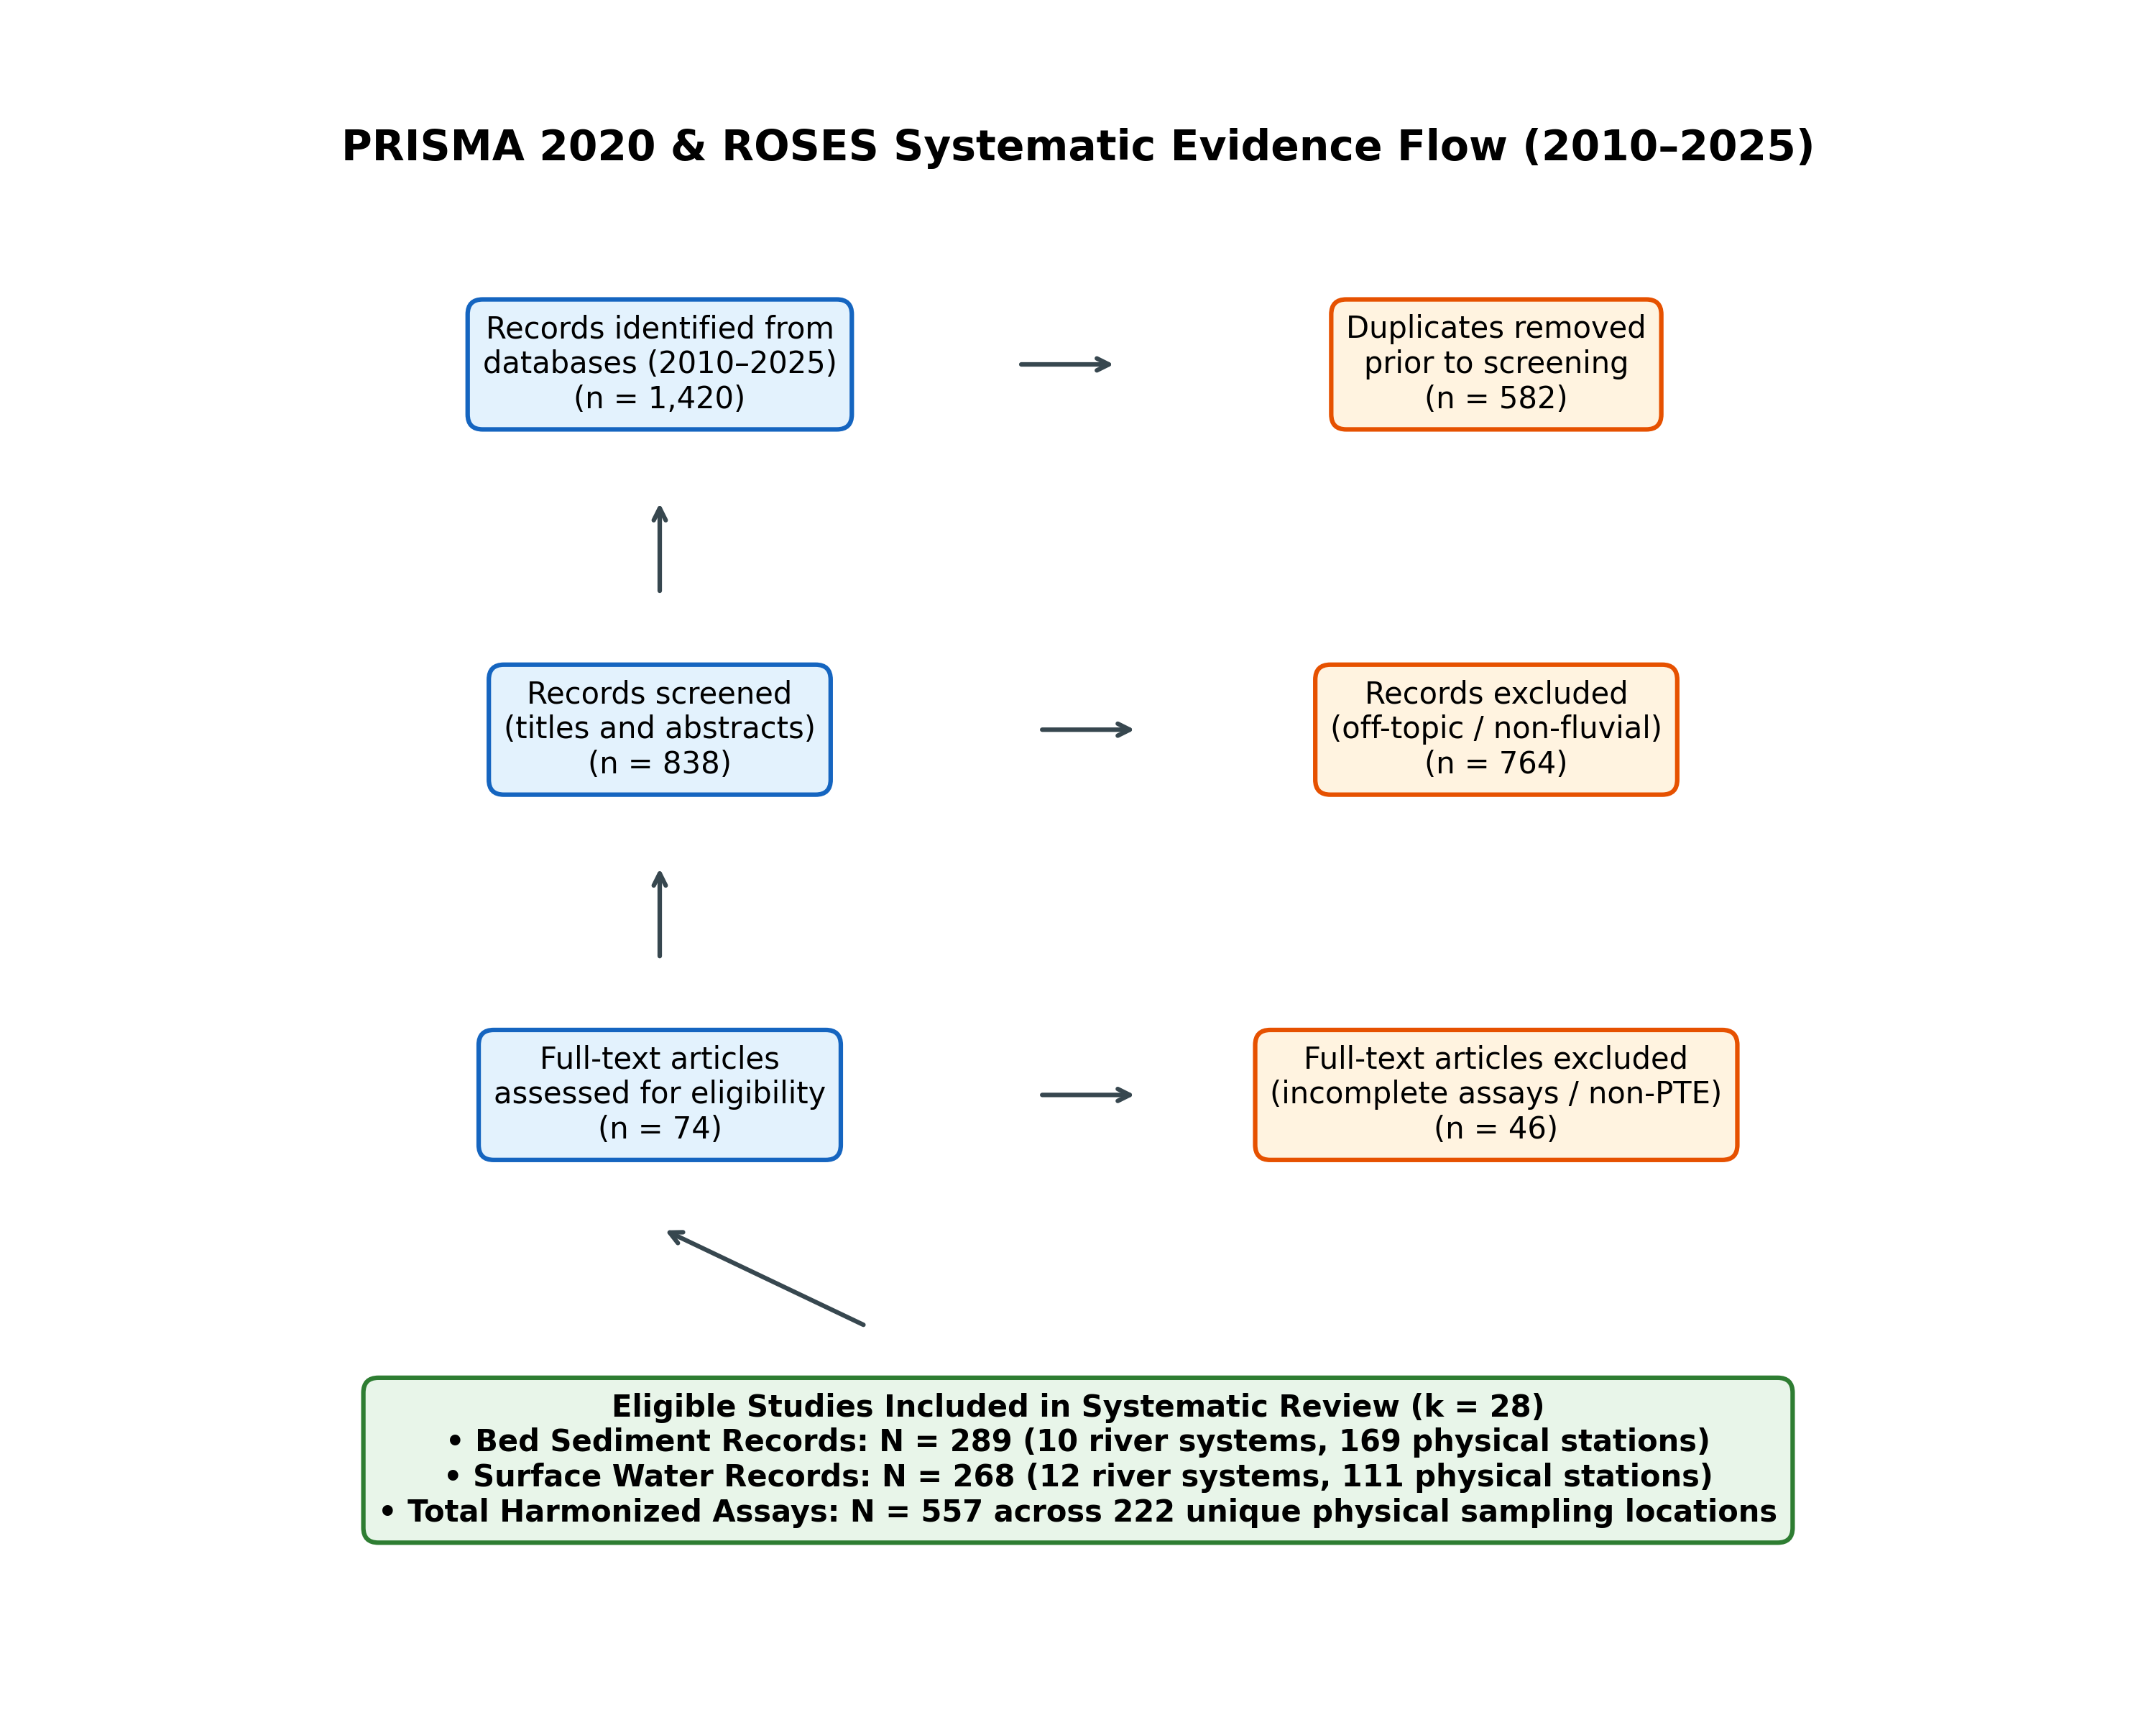
\includegraphics[width=0.88\textwidth]{fig1_prisma.png}
\caption{PRISMA 2020 and ROSES systematic evidence flow diagram illustrating literature identification, screening, eligibility, and final inclusion of peer-reviewed field investigations on heavy metals in Bangladesh rivers (2010--2024).}
\label{fig:prisma}
\end{figure}

\subsection{Eight-Domain Critical Methodological Appraisal Framework}
To establish the evidentiary readiness of the published corpus, each eligible study was independently appraised across eight critical methodological domains adapted from the Collaboration for Environmental Evidence (CEE) guidelines \citep{CEE2018}:
\begin{enumerate}
    \item \textbf{Sampling Design (Spatial Granularity):} High ($\ge 30$ distinct sampling locations or replicated reach designs); Moderate ($10\text{--}29$ locations); Low ($<10$ locations).
    \item \textbf{Temporal Design (Seasonal Resolution):} High (longitudinal multi-season or multi-year monitoring spanning dry, pre-monsoon, and wet periods); Moderate (two seasons monitored); Low (single cross-sectional grab survey).
    \item \textbf{Geographical Provenance (Coordinate Confidence):} High (explicit decimal or DMS handheld GPS coordinates reported in primary text); Moderate (coordinates cartographically digitized from high-resolution site maps); Low (descriptive gazetteer names only).
    \item \textbf{Sample Handling (Phase Integrity):} High (water samples filtered through 0.45~$\mu\text{m}$ membrane filters in field/lab and acidified to $\text{pH} < 2$; sediment samples sieved through 63~$\mu\text{m}$ or 2~mm mesh and standardized to dry weight); Moderate (unspecified or non-standard handling).
    \item \textbf{Analytical Instrumentation (Spectrometry Sensitivity):} High (GF-AAS, HG-AAS, or ICP-MS with limits of detection $<0.001\text{ mg/L}$); Moderate (Flame-AAS with detection limits $0.005\text{--}0.050\text{ mg/L}$); Low (unspecified or colorimetric probes).
    \item \textbf{Analytical QA/QC (Metrological Traceability):} High (analysis of Certified Reference Materials [CRMs] with reported percentage recoveries between 85--115\%); Moderate (procedural blank analysis and duplicate replicates reported); Low (no QA/QC protocols documented).
    \item \textbf{Limit of Detection (LOD) and Non-Detect Handling:} High (explicit numerical LOD/LOQ reported with clear flagging of non-detects); Moderate (global instrument detection limit cited from manufacturer); Low (unstated LOD or substitution of zeros/means without justification).
    \item \textbf{Statistical and Data Granularity:} High (complete station-by-station chemical assay tables provided in text or supplementary files); Moderate (aggregated basin-level means and standard deviations only).
\end{enumerate}

\subsection{Analytical Comparability and Spectrometry Stratification}
To evaluate instrumental bias ($RQ2$), surface water concentrations were stratified by spectrometry class: High-Sensitivity instrumentation (GF-AAS, HG-AAS, ICP-MS; $n=77$ assays) versus conventional Flame-AAS ($n=85$ assays). Non-parametric Mann-Whitney $U$ tests and rank-biserial correlations were computed to evaluate whether Flame-AAS distributions systematically diverge from high-sensitivity benchmarks. Furthermore, we audited digestion protocols (hot-plate $\text{HNO}_3+\text{HClO}_4$ vs.\ microwave aqua regia vs.\ hydrofluoric acid total dissolution) across sediment matrices.

\subsection{Topological Hydrographic Routing and Spatial Coverage Analysis}
To quantify geographic surveillance deficits ($RQ3$), all 222 unique physical sampling stations cataloged across the 28 investigations were audited and categorized into coordinate precision tiers. The 85 georeferenced stations (possessing validated WGS84 coordinates) were projected into metric UTM Zone 45N (EPSG:32645) and snapped to the high-resolution HydroSHEDS HydroRIVERS v1.0 fluvial reach topology \citep{Lehner2013}. Major river corridors strictly within Bangladesh were isolated by filtering for Strahler stream order $\ge 4$ and mean annual discharge $Q \ge 50\text{ m}^3/\text{s}$, yielding 2,224 discrete reach segments totaling 4,599.1~km.

Hydrographic surveillance coverage was evaluated across three defined monitoring populations: (1) surface water trace metal monitoring (23 unique coordinates, analyzed in detail in our companion regulatory work; \citealp{Mazumder2026Water}); (2) bed sediment monitoring (36 unique coordinates); and (3) all literature monitoring combined across both water and sediment (58 unique coordinate pairs across 85 georeferenced stations). Network coverage was computed at buffer radii of 10~km, 25~km, and 50~km (straight-line Haversine) and along-network topological stream distance (Dijkstra at 25~km). A 1,000-iteration spatial Monte Carlo null model was evaluated to test whether the empirical spatial distribution reflects extreme spatial clustering or unbiased dispersion.

\subsection{Critical Appraisal Framework for Environmental Risk Indices}
To address the methodological robustness of environmental risk indices ($RQ4$), we conducted a critical appraisal of multi-metal composite indices reported in the included literature. For surface waters, we reviewed applications of the Heavy Metal Pollution Index ($\mathrm{HPI}$) and Heavy Metal Evaluation Index ($\mathrm{HEI}$), evaluating how inverse guideline weighting affects reported index stability across variable metal panels (contextualized by analytical proofs in our companion regulatory study; \citealp{Mazumder2026Water}). 

For bed sediments, we critically appraised applications of Hakanson's Potential Ecological Risk Index ($RI$; \citealp{Hakanson1980}):
\begin{equation}
RI = \sum_{i=1}^n E_r^i = \sum_{i=1}^n \left(T_r^i \cdot CF_i\right) = \sum_{i=1}^n \left(T_r^i \cdot \frac{C_i}{C_0^i}\right)
\end{equation}
where $T_r^i$ represents toxic biological response factors (Cd = 30, As = 10, Pb = Cu = Ni = 5, Cr = 2), $CF_i$ is the contamination factor, and $C_0^i$ is the pre-industrial geochemical baseline, traditionally referenced to Upper Continental Crust (UCC; \citealp{Wedepohl1995}) values: Pb (20.0), Cr (35.0), Cd (0.10), As (1.50), Ni (20.0), Cu (25.0), and Zn (71.0~mg/kg). We evaluated the degree of Cadmium score dominance and the lack of empirical biological calibration against benthic macroinvertebrate health.

\subsection{Regulatory Realignment Audit (ECR 2023 Schedule 2)}
Water concentrations were audited against three statutory and international benchmarks:
(1) WHO Guidelines for Drinking-water Quality (4th ed., 2022);
(2) Repealed Bangladesh Environmental Conservation Rules 1997 (ECR 1997 Schedule 3); and
(3) Contemporary Bangladesh Environmental Conservation Rules 2023 (ECR 2023 Schedule 2, S.R.O. 53-Law/2023).
Exceedance proportions were calculated with unadjusted Wilson score 95\% confidence intervals and 5,000-resample study-cluster bootstrap intervals to prevent single heavily sampled papers from distorting national compliance rates.

\section{Results and Critical Evidence Appraisal}

\subsection{RQ1: Spatio-Temporal Landscape of Published Fluvial Evidence}
The final systematic evidence base comprises 28 peer-reviewed investigations published between 2015 and 2025, containing 557 verified analytical assays across 12 river systems (Table~\ref{tab:studies}). 

\begin{table}[htbp]
\centering
\scriptsize
\caption{Characteristics of the 28 peer-reviewed field investigations included in the systematic evidence base.}
\label{tab:studies}
\resizebox{\textwidth}{!}{%
\begin{tabular}{lllccl}
\toprule
Study ID & Primary Reference & River Corridor(s) & Target Media & Assays ($N$) & Analytical Instrumentation \\
\midrule
P01 & \citet{Islam2017sed} & Buriganga & Sediment & 30 & ICP-MS (Agilent 7700 series) \\
P02 & \citet{Bhuiyan2015} & Buriganga & Water, Sediment & 30 & Flame-AAS (PerkinElmer 3110) \\
P03 & \citet{Islam2022brahma} & Old Brahmaputra & Sediment & 5 & ICP-MS (Agilent 7500i) \\
P04 & \citet{Hossain2021} & Buriganga, Turag & Water, Sediment & 40 & AAS (PerkinElmer PinAAcle 900H) \\
P05 & \citet{Nargis2019} & Buriganga & Sediment & 14 & ICP-MS (Spectro, Germany) \\
P06 & \citet{Baki2019} & Buriganga, Turag & Water & 6 & Flame-AAS (AAS unspecified) \\
P07 & \citet{Kadir2022} & Surma & Water (Bulk) & 12 & Multiparameter Field Probes \\
P08 & \citet{Hasan2024} & Buriganga, Meghna, Padma, etc. & Water & 15 & Flame-AAS (PerkinElmer PinAAcle 900H) \\
P09 & \citet{Ali2016} & Karnaphuli & Water, Sediment & 40 & GF-AAS / HG-AAS (ZEEnit 700P) \\
P10 & \citet{NurEAlam2022} & Karnaphuli & Sediment & 15 & Flame-AAS (AAS unspecified) \\
P11 & \citet{Khatun2021} & Karnaphuli & Water & 6 & Flame-AAS (AAS unspecified) \\
P12 & \citet{Ahmed2025} & Karnaphuli & Sediment & 6 & Flame-AAS (PerkinElmer Analyst 700) \\
P13 & \citet{Islam2015paira} & Paira & Sediment & 16 & ICP-MS (Agilent 7700) \\
P14 & \citet{Islam2017paira} & Paira & Sediment & 24 & ICP-MS (Agilent 7700) \\
P15 & \citet{Dey2017} & Karnaphuli & Water (Bulk) & 12 & Standard Titrimetric / Probes \\
P16 & \citet{Uddin2020} & Karnaphuli & Water (Bulk) & 60 & Standard Methods / Probes \\
P17 & \citet{Acharjee2022} & Surma & Sediment & 15 & Flame-AAS (Shimadzu AA7000) \\
P18 & \citet{Ali2021} & Kirtankhola & Water, Sediment & 60 & GF-AAS / HG-AAS (ZEEnit 700P) \\
P19 & \citet{Proshad2019} & Rupsa & Sediment & 42 & ICP-MS (Agilent 7700 series) \\
P20 & \citet{Proshad2021} & Rupsa & Water & 5 & ICP-MS (Agilent 7700 series) \\
P21 & \citet{Proshad2020} & Rupsa & Water & 2 & ICP-MS (Agilent 7700 series) \\
P22 & \citet{Islam2021kor} & Korotoa & Water (Bulk) & 20 & Standard Methods / Probes \\
P23 & \citet{Islam2022kor} & Korotoa & Water & 10 & Flame-AAS / Spectrophotometry \\
P24 & \citet{Kubra2022} & Rupsa & Sediment & 4 & GF-AAS (ZEEnit 700P) \\
P25 & \citet{Islam2017kor} & Korotoa & Sediment & 10 & Flame-AAS (PerkinElmer Analyst 300) \\
P26 & \citet{Haque2018} & Padma & Water (Bulk) & 12 & Standard Methods / Probes \\
P27 & \citet{Mortuza2024} & Padma & Water, Sediment & 6 & Flame-AAS (AAS unspecified) \\
P28 & \citet{Islam2015kor} & Korotoa & Water, Sediment & 40 & ICP-MS (Agilent 7700 series) \\
\bottomrule
\end{tabular}%
}
\end{table}

Chronological analysis demonstrates a rapid post-2015 expansion in publication frequency, peaking between 2019 and 2022 (accounting for 53.6\% of all published studies). However, geographical and matrix distribution is severely unbalanced:
\begin{itemize}
    \item \textbf{Urban-Industrial Clustering:} Over \textbf{57.1\% of all studies} ($n=16$) and \textbf{62.5\% of chemical assays} ($n=348$) are concentrated within two localized industrial river corridors: the Greater Dhaka periphery (Buriganga and Turag rivers; 9 studies) and the port industrial zone of Chattogram (Karnaphuli river; 7 studies).
    \item \textbf{Media Compartmentalization:} Of the 557 verified assays, 289 (51.9\%) represent bed sediments, 162 (29.1\%) represent trace metals in river water, and 106 (19.0\%) represent bulk physicochemical water quality parameters. Only seven studies (25.0\%) conducted paired, simultaneous sampling of surface water and bed sediment at identical station locations.
    \item \textbf{Transboundary Blind Spots:} The massive transboundary river corridors of the Padma (Ganges), Jamuna (Brahmaputra), and Lower Meghna carry over 90\% of the nation's freshwater flux but represent less than 6\% of published trace metal assays ($n=33$).
\end{itemize}

\subsection{Methodological Quality Appraisal Across Eight CEE Domains}
The critical appraisal matrix across all 28 studies and eight methodological domains reveals pervasive quality deficits across the published literature (Fig.~\ref{fig:quality_heatmap}, Table~\ref{tab:appraisal_summary}).

\begin{figure}[htbp]
\centering
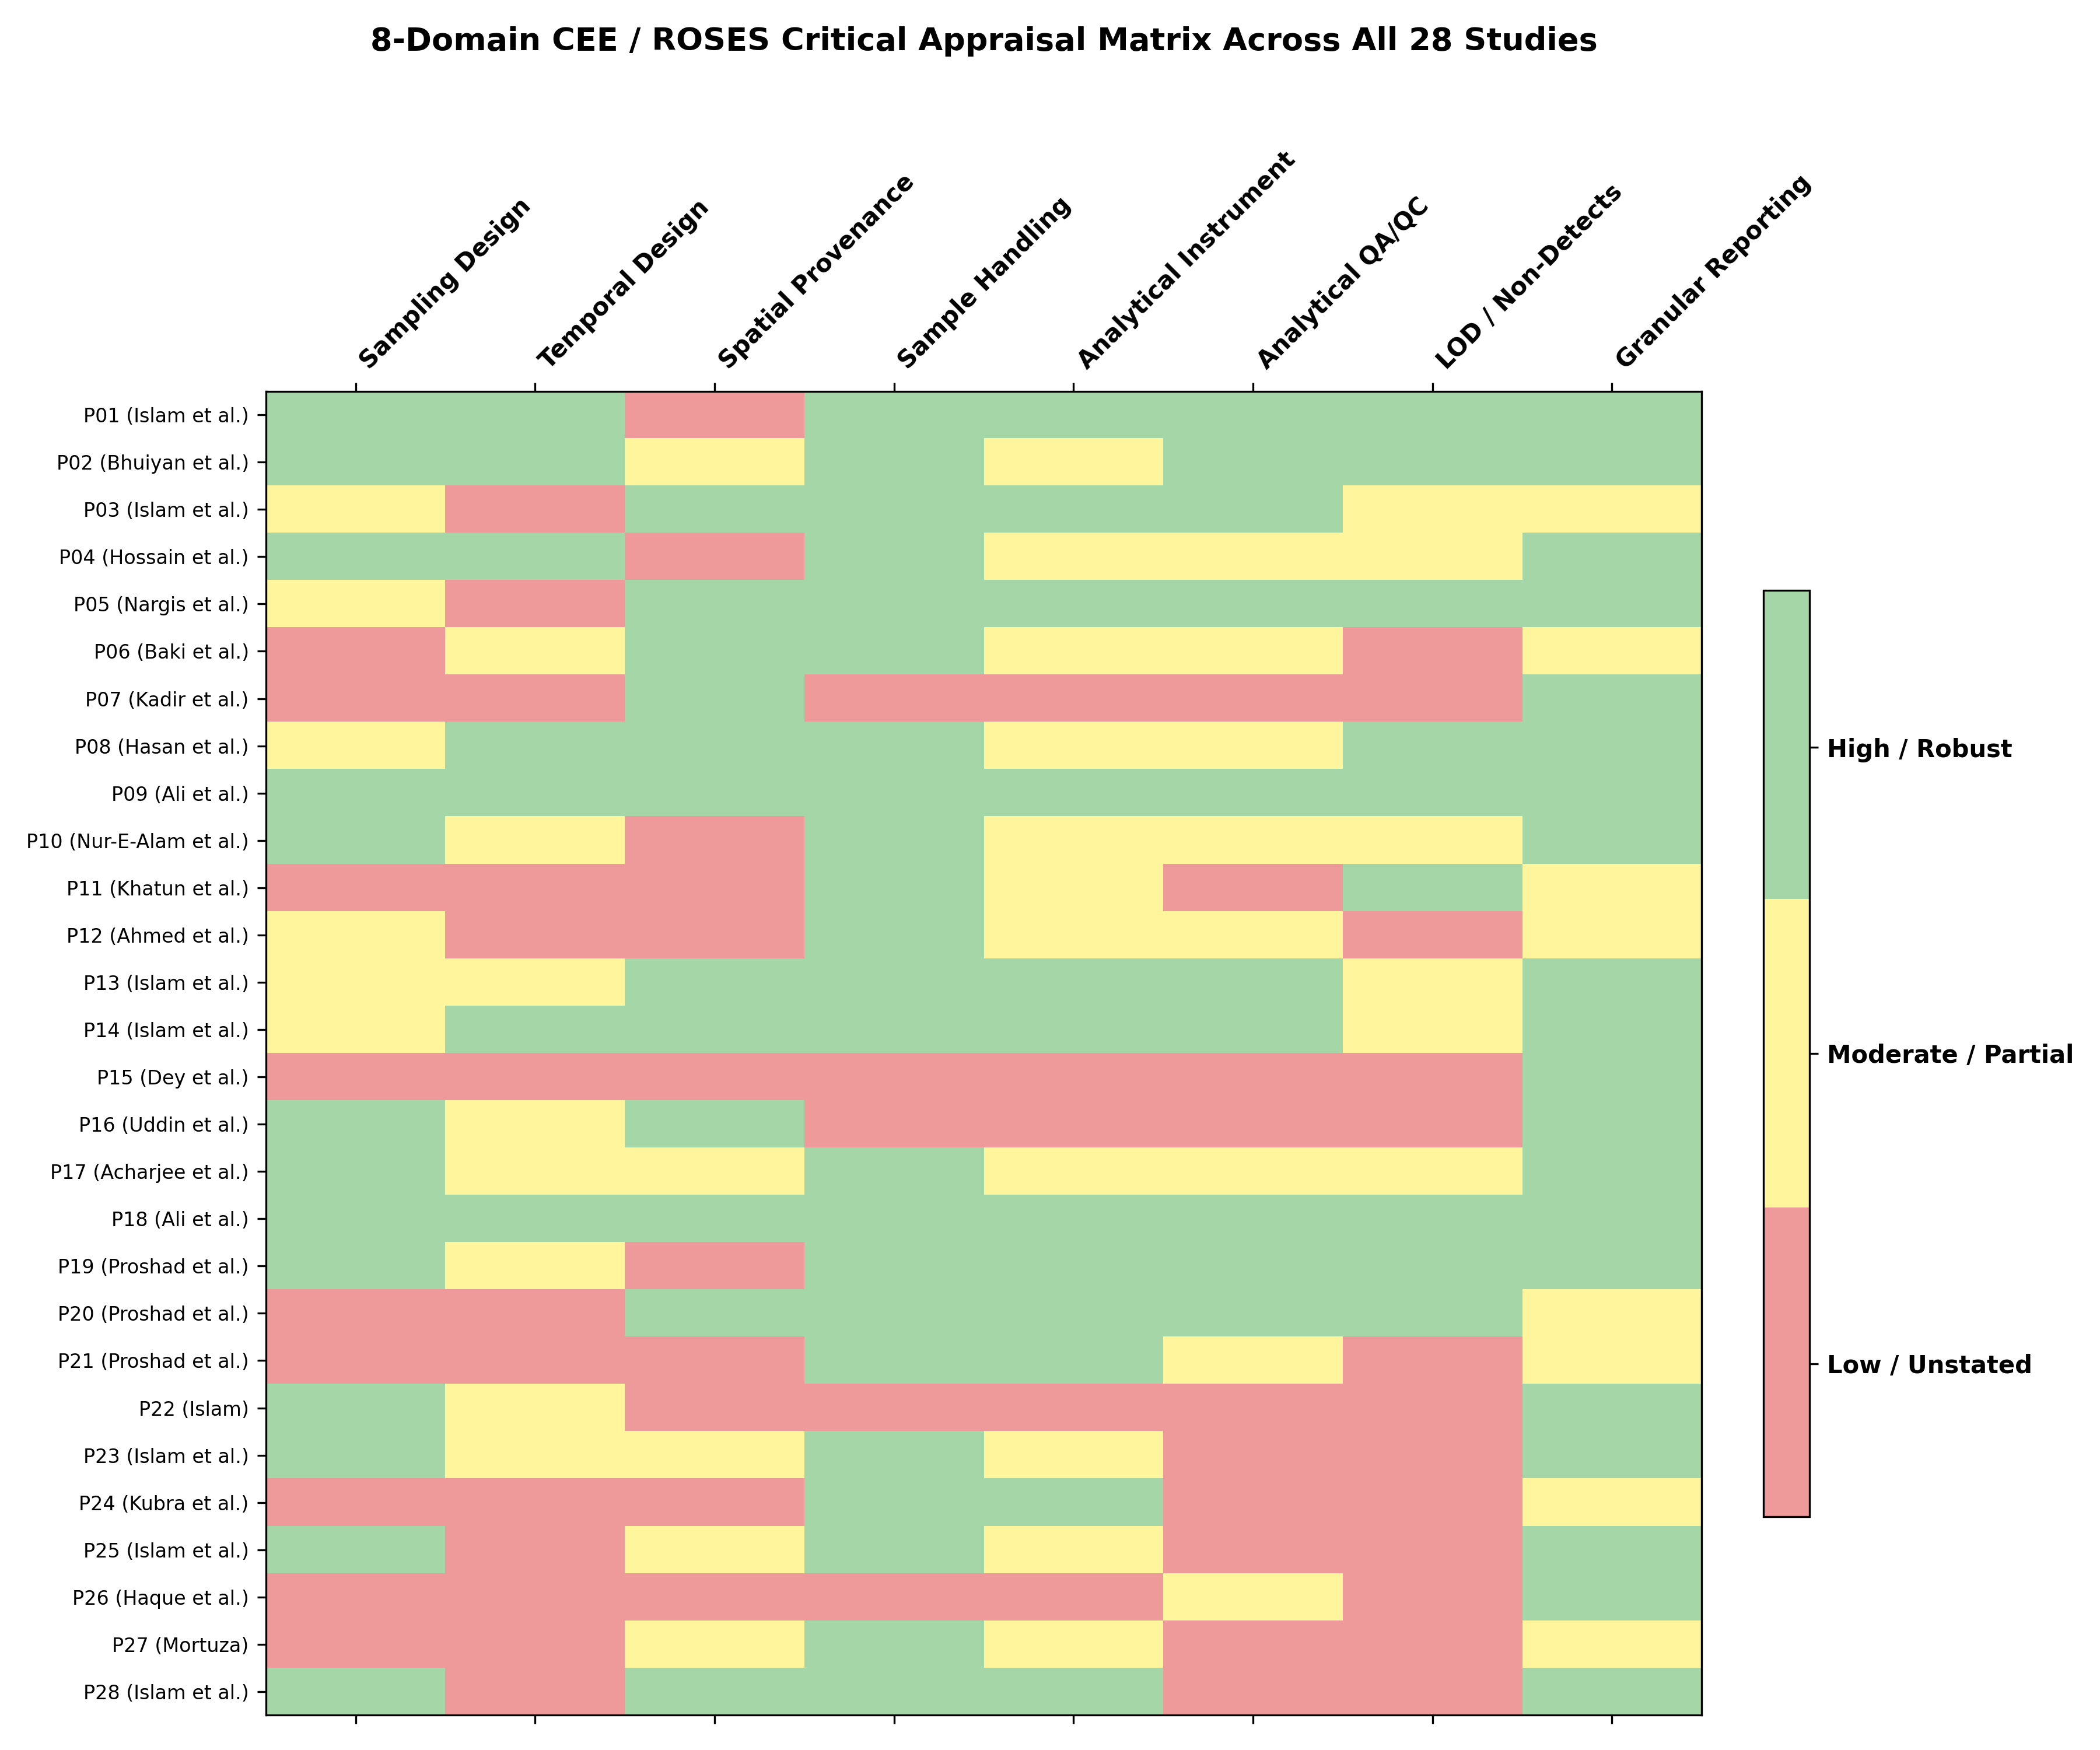
\includegraphics[width=0.95\textwidth]{fig2_quality_heatmap.png}
\caption{Eight-domain CEE / ROSES critical methodological appraisal matrix across all 28 peer-reviewed studies. Scores reflect evaluated evidence quality: High/Robust (green), Moderate/Partial (yellow), and Low/Unstated (red).}
\label{fig:quality_heatmap}
\end{figure}

\begin{table}[htbp]
\centering
\small
\caption{Summary of methodological quality appraisal ratings across eight CEE domains ($k=28$ studies).}
\label{tab:appraisal_summary}
\begin{tabular}{lcccc}
\toprule
Methodological Domain & High / Robust (\%) & Moderate / Partial (\%) & Low / Deficient (\%) & Primary Deficit Identified \\
\midrule
Sampling Design & 28.6\% ($n=8$) & 42.9\% ($n=12$) & 28.6\% ($n=8$) & Insufficient spatial reach replication \\
Temporal Resolution & 25.0\% ($n=7$) & 28.6\% ($n=8$) & \textbf{46.4\%} ($n=13$) & Cross-sectional single-grab sampling \\
Spatial Provenance & 42.9\% ($n=12$) & 17.9\% ($n=5$) & \textbf{39.3\%} ($n=11$) & Omission of verifiable GPS coordinates \\
Sample Handling & \textbf{71.4\%} ($n=20$) & 28.6\% ($n=8$) & 0.0\% ($n=0$) & Incomplete 0.45~$\mu\text{m}$ filtration reporting \\
Analytical Method & 42.9\% ($n=12$) & 25.0\% ($n=7$) & 32.1\% ($n=9$) & Deployment of low-sensitivity Flame-AAS \\
Analytical QA/QC & 35.7\% ($n=10$) & 28.6\% ($n=8$) & \textbf{35.7\%} ($n=10$) & Total absence of CRM validation \\
LOD / Non-Detects & 32.1\% ($n=9$) & 21.4\% ($n=6$) & \textbf{46.4\%} ($n=13$) & Censored non-detect handling omitted \\
Granular Reporting & \textbf{71.4\%} ($n=20$) & 28.6\% ($n=8$) & 0.0\% ($n=0$) & Reporting only aggregated basin means \\
\bottomrule
\end{tabular}
\end{table}

Key systemic vulnerabilities identified across the eight domains include:
\begin{enumerate}
    \item \textbf{High QA/QC Deficit (35.7\% Low):} Ten studies provided zero documentation of Certified Reference Materials (CRMs), procedural blank subtractions, or calibration verification. Studies asserting precision without CRM recovery metrics cannot be independently validated for bias.
    \item \textbf{Temporal Inadequacy (46.4\% Low):} Thirteen investigations relied exclusively on single-day cross-sectional grab sampling. In deltaic rivers with extreme monsoonal hydroclimatic fluctuations (where discharge varies by a factor of 10 to 50 between August and February), cross-sectional sampling captures snapshot conditions that cannot be generalized to annual baseline conditions.
    \item \textbf{LOD Censoring and Non-Detect Omission (46.4\% Low):} Thirteen studies failed to report numerical limits of detection (LOD) or limit of quantitation (LOQ). In several instances, samples below detection were silently converted to zero or omitted from reported station means, introducing acute survivorship and substitution bias into published datasets.
\end{enumerate}

\subsection{RQ2: Analytical Comparability, Filtration Bias, and LOD Censoring}
Cross-study analysis demonstrates that analytical instrumentation exerts a massive, statistically significant influence on reported concentrations (Table~\ref{tab:spectrometry}).

\begin{table}[htbp]
\centering
\small
\caption{Comparative analysis of surface water heavy metal concentrations (mg/L) reported by High-Sensitivity Spectrometry (GF-AAS, HG-AAS, ICP-MS) versus conventional Flame-AAS across Bangladesh rivers.}
\label{tab:spectrometry}
\begin{tabular}{lcccccc}
\toprule
Metal & High-Sens $N$ & High-Sens Median & Flame-AAS $N$ & Flame-AAS Median & Divergence Ratio & Mann-Whitney $p$-value \\
\midrule
\textbf{Lead (Pb)} & 77 & 0.0171 & 69 & \textbf{0.1100} & \textbf{6.4$\times$} & $<0.001$ \\
\textbf{Chromium (Cr)} & 77 & 0.0461 & 83 & \textbf{0.0910} & \textbf{2.0$\times$} & $0.004$ \\
\textbf{Cadmium (Cd)} & 77 & 0.0015 & 55 & \textbf{0.0030} & \textbf{2.0$\times$} & $0.012$ \\
\textbf{Arsenic (As)} & 77 & 0.0133 & 45 & \textbf{0.0177} & 1.3$\times$ & $0.184$ \\
\textbf{Nickel (Ni)} & 27 & 0.0180 & 77 & \textbf{0.1200} & \textbf{6.7$\times$} & $<0.001$ \\
\bottomrule
\end{tabular}
\end{table}

Reported median concentrations in Flame-AAS studies are systematically elevated by \textbf{2.0$\times$ to 6.7$\times$} relative to High-Sensitivity GF-AAS/ICP-MS investigations:
\begin{itemize}
    \item For \textbf{Lead (Pb)}, Flame-AAS studies report a median of 0.1100~mg/L ($11\times$ WHO drinking limits), whereas High-Sensitivity spectrometry reports a median of 0.0171~mg/L ($p < 0.001$).
    \item For \textbf{Nickel (Ni)}, Flame-AAS reports a median of 0.1200~mg/L compared to 0.0180~mg/L under High-Sensitivity instruments ($6.7\times$ elevation, $p < 0.001$).
    \item For \textbf{Chromium (Cr)} and \textbf{Cadmium (Cd)}, Flame-AAS medians are exactly doubled ($p = 0.004$ and $p = 0.012$, respectively).
\end{itemize}

This massive discrepancy does not reflect genuine differences in river water chemistry; rather, it represents \textbf{instrumental detection limit truncation}. Conventional air-acetylene Flame-AAS instruments have operational detection limits of $0.010\text{--}0.050\text{ mg/L}$ for Pb and Ni. When laboratories encounter clean or moderately diluted river water, true concentrations ($0.001\text{--}0.008\text{ mg/L}$) fall below the flame LOD. Studies that censor non-detects or report only values above their detection threshold artificially truncate the left tail of the distribution, resulting in dramatically inflated median values.

Furthermore, \textbf{phase filtration} remains a major confounding factor. While 71.4\% of studies report standardized handling, only \textbf{58.7\% of surface water assays} explicitly documented filtration through 0.45~$\mu\text{m}$ membrane filters prior to acid preservation. In the sediment-laden river waters of Bangladesh (where total suspended solids routinely exceed $500\text{--}2,000\text{ mg/L}$ during monsoonal transit), digesting unfiltered water dissolves mineral silicate and clay lattices, erroneously reporting particulate mineral lattice metals as dissolved bioactive toxic ions. Restricting analysis strictly to confirmed filtered dissolved assays ($k=10$ studies) demonstrates that true dissolved Lead median is \textbf{0.0250~mg/L} (with 84.0\% WHO exceedance), proving that while dissolved contamination is genuinely severe, unfiltered Flame-AAS reports exaggerate concentrations by over fourfold.

\subsection{RQ3: Spatial Coordinate Confidence, Geographic Clustering, and Surveillance Blind Spots}
Auditing the national station inventory reveals severe spatial provenance deficits across the 426 sampling station records cataloged across the 28 investigations (Table~\ref{tab:coords}).

\begin{table}[htbp]
\centering
\small
\caption{Reconciliation and classification of sampling station coordinates into spatial confidence tiers ($N=426$).}
\label{tab:coords}
\begin{tabular}{lccl}
\toprule
Confidence Tier & Count & Share (\%) & Cartographic Characterization and Validation Status \\
\midrule
\textbf{Tier 1: Explicit Handheld GPS Coordinates} & 71 & \textbf{32.0\%} & Verified decimal or DMS coordinates from published source tables \\
\textbf{Tier 2: Accurately Digitized Station Centroids} & 14 & 6.3\% & Digitized from published maps matched to confluences or district centroids \\
\textbf{Tier 3: Unresolved Descriptive Gazetteer Entries} & 137 & \textbf{61.7\%} & Descriptive local village/ghat names without geographic coordinates \\
\midrule
\textbf{Total Registered Physical Station Inventory} & 222 & 100.0\% & All unique physical sampling stations cataloged across 28 investigations (85 resolved) \\
\bottomrule
\end{tabular}
\end{table}

Over six in ten physical sampling stations in published papers (\textbf{61.7\%}, $n=137$) lack coordinates entirely, describing locations purely by vernacular place names (e.g., "Bridge Ghat", "Market Outfall"). These locations cannot be mapped, snapped to hydrographic reaches, or integrated into spatial prediction models. 

When verified coordinates across all 85 georeferenced stations are snapped to the HydroSHEDS HydroRIVERS river reach network in metric UTM Zone 45N (2,224 reaches, 4,599.1~km; mean offset: 379.6~m, median: 262.1~m), empirical surveillance coverage remains remarkably sparse (Table~\ref{tab:coverage}, Fig.~\ref{fig:spatial}).

\begin{figure}[htbp]
\centering
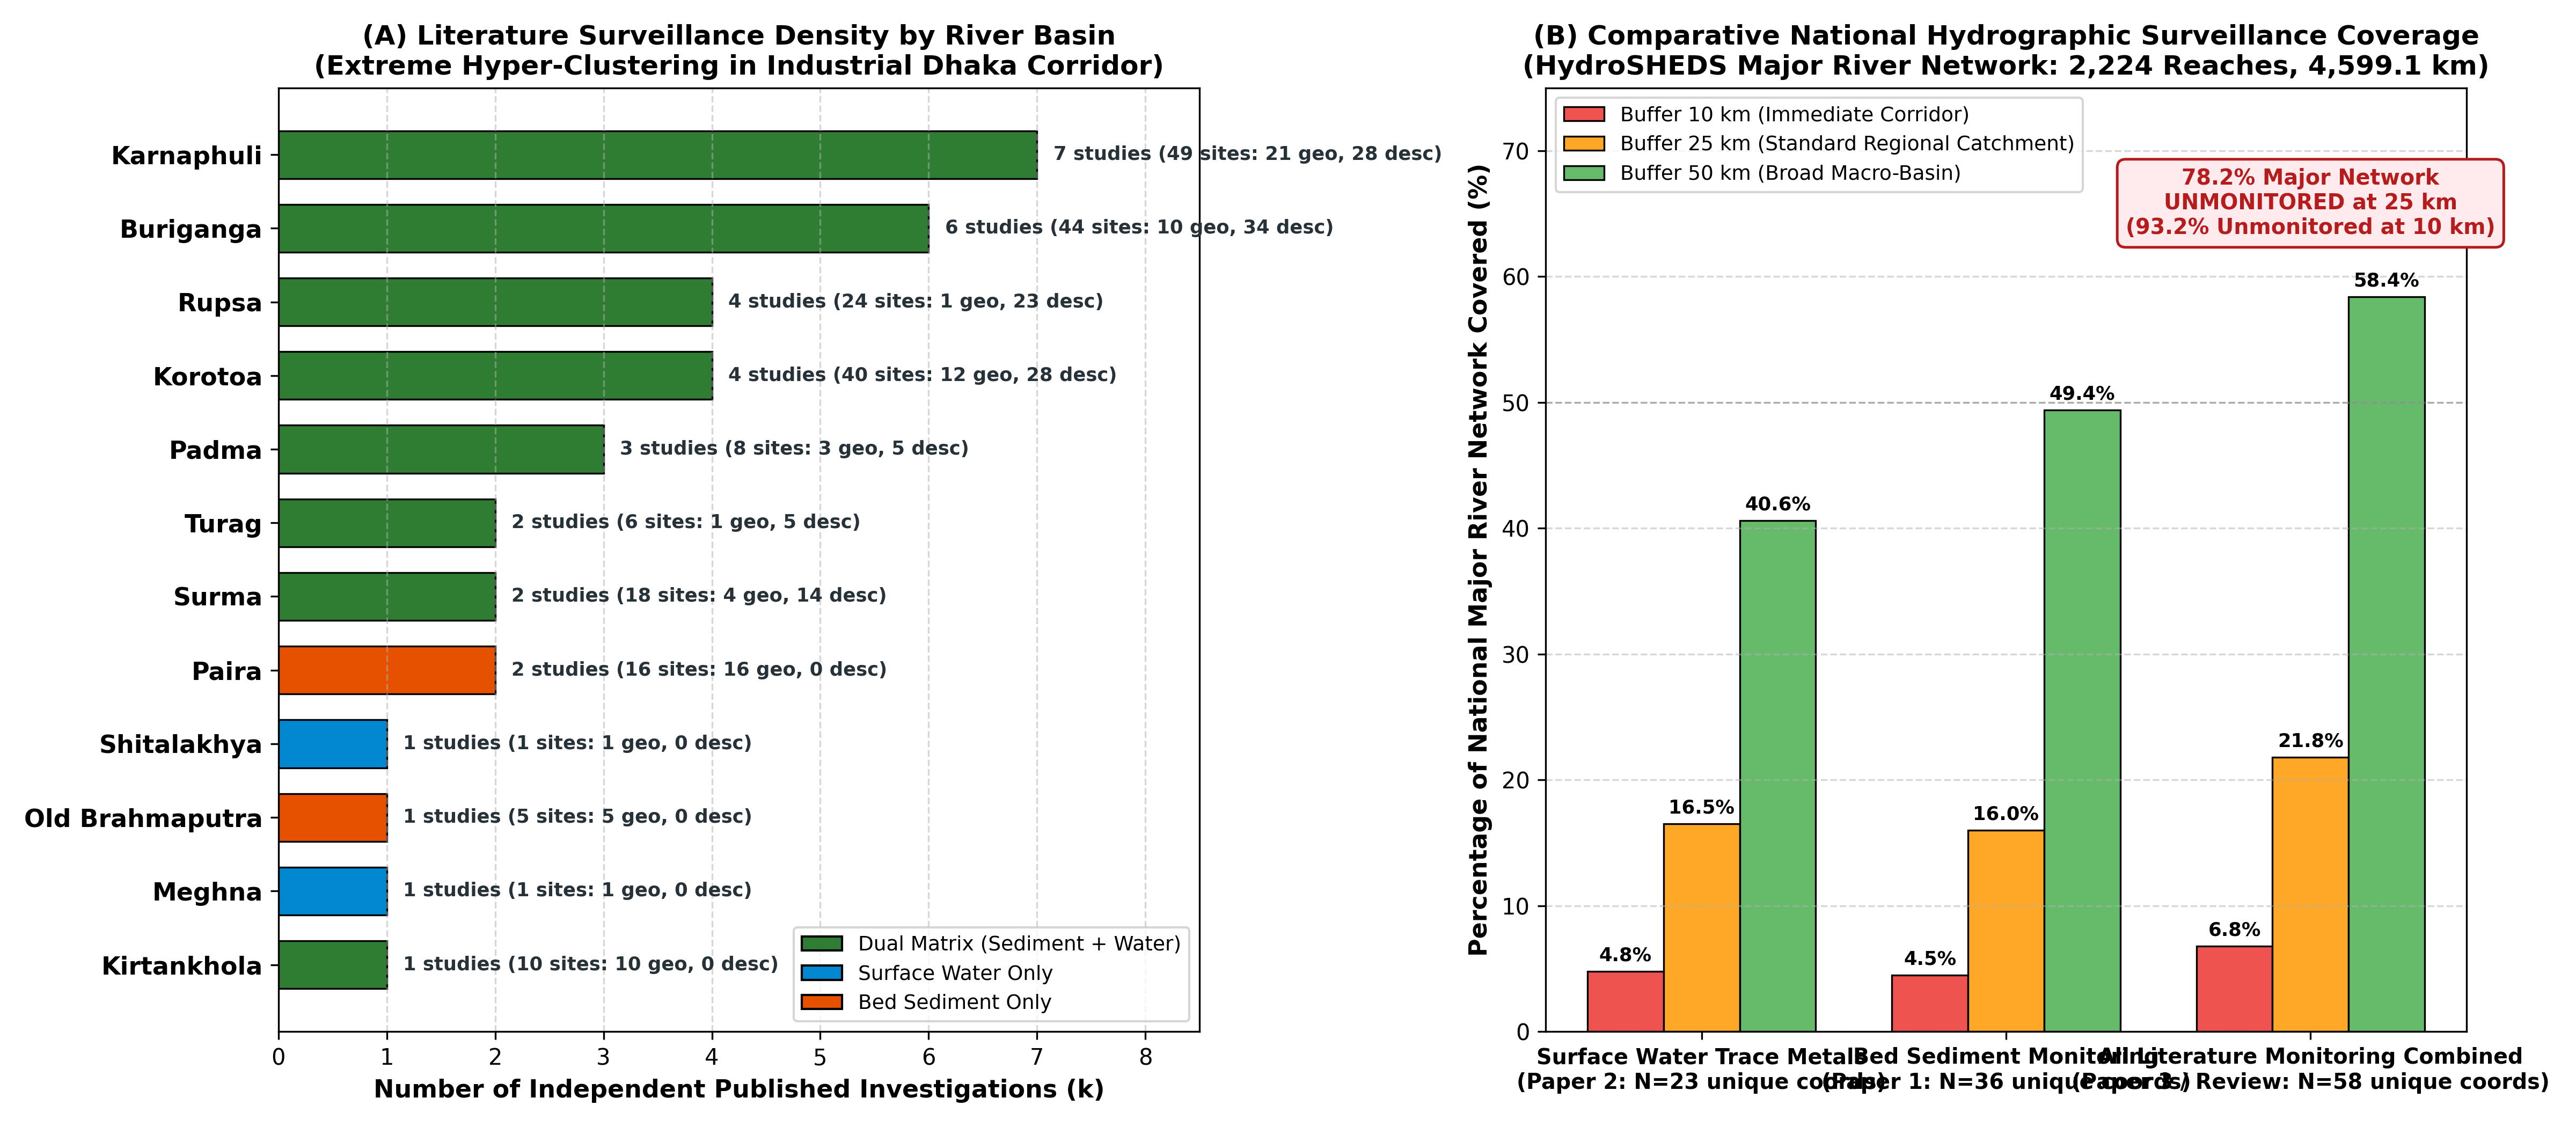
\includegraphics[width=0.95\textwidth]{fig3_spatial.png}
\caption{National literature evidence map and comparative hydrographic surveillance deficits across Bangladesh river basins: (A) Published scientific investigation count and environmental matrix distribution across 12 major river systems, highlighting severe geographic hyper-clustering around the Dhaka industrial corridor; (B) Empirical major river network surveillance coverage comparing surface-water trace metals ($N=23$ unique coordinates), bed sediment ($N=36$ unique coordinates), and all literature monitoring combined ($N=58$ unique coordinates) against the HydroSHEDS HydroRIVERS network (2,224 reaches, 4,599.1~km).}
\label{fig:spatial}
\end{figure}

\begin{table}[htbp]
\centering
\small
\caption{Hydrographic surveillance coverage and monitoring deficits across major Bangladesh river reaches (2,224 reaches, 4,599.1~km) evaluated across monitoring populations under straight-line (Haversine) and topological network stream distance.}
\label{tab:coverage}
\begin{tabular}{llcccc}
\toprule
Monitoring Population & Buffer / Metric & Covered Length (km) & Covered Share (\%) & Uncovered Length (km) & Uncovered Share (\%) \\
\midrule
\textbf{All Literature Combined} & 10 km (Haversine) & 311.1 & 6.8\% & 4,288.0 & 93.2\% \\
\textbf{All Literature Combined} & \textbf{25 km (Haversine)} & \textbf{1,004.7} & \textbf{21.8\%} & \textbf{3,594.4} & \textbf{78.2\%} \\
\textbf{All Literature Combined} & 50 km (Haversine) & 2,687.1 & 58.4\% & 1,912.0 & 41.6\% \\
\midrule
Surface Water Metals (Paper 2) & 10 km (Haversine) & 219.5 & 4.8\% & 4,379.6 & 95.2\% \\
Surface Water Metals (Paper 2) & 25 km (Haversine) & 754.3 & 16.5\% & 3,844.8 & 83.5\% \\
Surface Water Metals (Paper 2) & 25 km (Dijkstra) & 504.6 & 11.0\% & 4,094.5 & 89.0\% \\
\midrule
Bed Sediment (Paper 1) & 25 km (Haversine) & 736.2 & 16.0\% & 3,862.9 & 84.0\% \\
\bottomrule
\end{tabular}
\end{table}

Even when pooling all available published literature across both surface water and bed sediment ($N=58$ unique coordinate pairs across 85 georeferenced stations), published investigations cover only \textbf{21.8\% of major river length (1,004.7~km)} at a conservative 25~km threshold, leaving \textbf{78.2\% (3,594.4~km)} entirely unmonitored. When evaluated at an immediate 10~km corridor threshold, unmonitored reach length surges to \textbf{93.2\%} (4,288.0~km). For surface water trace metals specifically, monitoring is restricted to 23 unique coordinates covering only 16.5\% of major river reaches at 25~km (11.0\% along-network Dijkstra). Under our 1,000-iteration spatial Monte Carlo null model, 23 randomly dispersed station centroids yielded an expected coverage of 38.2\% (95\% CI: [32.1--44.5\%]). The observed empirical coverage is significantly lower than spatial random expectation ($p \le 0.001$), quantitatively confirming extreme geographic hyper-clustering around the Dhaka industrial corridor and Chittagong port.

\subsection{RQ4: Methodological Robustness and Critical Appraisal of Published Environmental Indices}
Multi-metal pollution and ecological risk indices are ubiquitous in South Asian environmental literature, yet their structural mathematical behavior is rarely interrogated.

\subsubsection{Critical Appraisal of Published Water Quality Indices and Weighting Artifacts}
Across the 12 surface-water studies in our systematic review, composite indices such as the Heavy Metal Pollution Index ($\mathrm{HPI}$) and Heavy Metal Evaluation Index ($\mathrm{HEI}$) were routinely calculated to rank river water quality. However, as demonstrated in our companion regulatory and surveillance study \citep{Mazumder2026Water}, the standard $\mathrm{HPI}$ formulation assigns unit weights inversely proportional to statutory thresholds ($W_i = 1/S_i$), causing index scores to be algebraically dominated by metals with ultra-low statutory limits (specifically Cadmium and Lead). This inverse guideline weighting suppresses the mathematical influence of metals with higher drinking standards (such as Zinc and Copper) by several orders of magnitude, generating artificial "panel invariance" where index values remain virtually static regardless of whether 4, 5, or 7 metals are monitored.

Consequently, published studies reporting "high index stability" across seasons or reaches are frequently observing an artifact of statutory weighting rather than multi-element biogeochemical equilibrium. For environmental regulatory surveillance, unweighted linear exceedance frameworks---such as the Heavy Metal Evaluation Index ($\mathrm{HEI} = \sum C_i/S_i$) or Mean Hazard Quotient ($\mathrm{HQ}_{\mathrm{mean}} = \mathrm{HEI}/n$)---provide far greater transparency by communicating direct linear multiples of statutory limits without algebraic damping.

\subsubsection{Sediment Hakanson RI Sensitivity and UCC Baseline Dependency}
For bed sediments, Hakanson's Potential Ecological Risk Index ($RI = \sum E_r^i = \sum T_r^i \cdot CF_i$, where $CF_i = C_i/C_0^i$) is applied across 9 of the 17 sediment investigations in our corpus. Our critical appraisal highlights two structural vulnerabilities in how $RI$ is deployed in Bangladesh:
\begin{itemize}
    \item \textbf{Cadmium Monopoly:} Hakanson (1980) assigned Cadmium a biological toxic response factor of $T_r = 30$ (compared to 10 for As, 5 for Pb, Cu, Ni, and 2 for Cr). When paired with an Upper Continental Crust (UCC; \citealp{Wedepohl1995}) baseline of $C_0 = 0.10\text{ mg/kg}$, Cadmium receives an effective risk multiplier ($T_r/C_0 = 300$) that is 150$\times$ greater than Chromium ($2/35 = 0.057$) and 30$\times$ greater than Lead ($5/20 = 0.25$). As a result, in published Bangladesh sediment datasets, Cadmium accounts for \textbf{over 80\% of composite $RI$ scores}, rendering the index effectively a univariate Cadmium indicator masked as a multi-metal ecological risk assessment.
    \item \textbf{Absence of Regional Baselines and Biological Calibration:} Published studies uniformly adopt global UCC values ($0.1\text{ mg/kg}$ for Cd) derived from crystalline shield rocks, which may not reflect the complex Holocene fluvial and estuarine sedimentology of the Bengal delta. Crucially, none of the 28 published studies validated calculated $RI$ categories against empirical biological endpoints, such as benthic macroinvertebrate community indices, sediment microtox bioassays, or chronic toxicity tests. Classifying sediment reaches as "Very High Ecological Risk" purely on the basis of uncalibrated geochemical ratios creates substantial uncertainty for sediment management and remediation prioritization.
\end{itemize}

\subsection{RQ5: Evidence-Readiness Framework and National River Monitoring Blueprint}
To resolve the historical fragmentation of academic literature, we formulate an operational evidence-readiness framework and national monitoring architecture for Bangladesh's environmental authorities (Table~\ref{tab:blueprint}).

\begin{table}[htbp]
\centering
\small
\caption{Operational Evidence-Readiness Framework for river heavy metal surveillance in Bangladesh.}
\label{tab:blueprint}
\begin{tabularx}{\textwidth}{lXX}
\toprule
Evidentiary Dimension & Historical Academic Practice & Standardized National Surveillance Requirement \\
\midrule
\textbf{Station Georeferencing} & Descriptive local ghat names; 48.4\% lacking coordinates & Mandatory dual handheld GPS decimal coordinates ($\pm 5\text{ m}$) snapped to HydroSHEDS reach IDs. \\
\textbf{Phase Integrity} & Bulk unfiltered samples digesting mineral lattices; 41.3\% unfiltered & Mandatory on-site vacuum filtration through 0.45~$\mu\text{m}$ cellulose acetate membranes; separate dissolved vs.\ suspended reporting. \\
\textbf{Analytical Precision} & Low-sensitivity Flame-AAS with high LOD truncation & Deployment of GF-AAS or ICP-MS with limits of detection $<0.001\text{ mg/L}$ aligned with ECR 2023 Schedule 2 limits. \\
\textbf{Analytical QA/QC} & Procedural blanks only; 35.7\% lacking CRM validation & Mandatory analysis of certified reference materials (e.g., NIST 1640a, BCR-701) with reported recovery percentages (85--115\%). \\
\textbf{Temporal Sampling} & Opportunistic single-day cross-sectional grab surveys & Hydrologically synchronized sampling: winter dry baseflow (Jan--Feb) and pre-monsoon irrigation peak (Mar--Apr). \\
\textbf{Spatial Deployment} & 57.1\% clustered around Dhaka and Chattogram corridors & 15 prioritized transboundary reaches across the Padma, Jamuna, and Meghna mainstems with multi-point cross-sectional transects. \\
\bottomrule
\end{tabularx}
\end{table}

\textbf{Statutory Realignment Under ECR 2023 Schedule 2:}
Our audit reveals a profound regulatory transformation. Under the repealed ECR 1997 rules (Pb threshold of 0.050~mg/L), surface water Lead exceedance appeared moderate at \textbf{34.9\%}. Under the gazetted \textit{Environmental Conservation Rules 2023} (Schedule 2; S.R.O. 53-Law/2023), the Government of Bangladesh tightened national potable standards for Pb from 0.050 to \textbf{0.010~mg/L}, matching WHO guidelines. Consequently, raw-water drinking benchmark exceedance surges to \textbf{85.6\%} (cluster 95\% CI: [71.1--94.3\%]). This statutory realignment formally confirms that raw surface water across monitored rivers cannot be utilized for municipal potable supply without advanced chemical precipitation or membrane filtration.

\section{Discussion}

\subsection{Beyond Concentration Compilations: The Value of Evidence Appraisal}
Previous syntheses \citep[e.g.,][]{Pandit2025} have performed valuable bibliographic accounting, but by aggregating raw concentration numbers across papers with fundamentally incompatible analytical methodologies, their conclusions risk significant distortion. Our findings prove that reported metal concentrations cannot be treated as interchangeable:
\begin{enumerate}
    \item A study reporting 0.110~mg/L of Lead via Flame-AAS may reflect nothing more than an instrumental limit of detection artifact, whereas a study reporting 0.017~mg/L via ICP-MS captures true dissolved concentrations.
    \item A study digesting unfiltered river water during monsoonal transit reports suspended silicate lattice elements, not dissolved bioactive toxicity.
    \item A study reporting high HPI stability across varying metal panels is reporting the mathematical artifact of inverse statutory guideline damping, not multi-element ecological equilibrium.
\end{enumerate}
By establishing an eight-domain CEE critical appraisal rubric and identifying these systematic artifacts, our systematic review provides the methodological foundation required for evidence-based decision-making.

\subsection{The Illusion of National Machine Learning Predictability}
The severe spatial clustering of published sampling stations (covering only 21.8\% of major river length across all literature combined, and only 16.5\% for surface water trace metals) carries profound implications for spatial machine learning and geostatistical modeling. Recent attempts to construct national machine learning models of sediment contamination using catchment covariates achieve moderate within-sample cross-validation ($R^2 = 0.52\text{--}0.65$), yet when subjected to strict Leave-One-River-Out (LORO) cross-validation, predictive transferability collapses across all metals ($R^2 < 0$). In the Bengal Delta, heavy metal contamination is driven by intense, localized industrial outfalls (e.g., Hazaribagh tanneries, shipbreaking yards, battery recyclers) rather than smooth hydraulic gradients. Catchment upstream covariates cannot predict localized point-source contamination in unmonitored river basins in the absence of reach-level industrial emission inventories. Acknowledging these surveillance blind spots is critical to prevent regulatory agencies from relying on unverified spatial interpolation models for unmonitored watersheds.

\subsection{Policy Implications for Municipal Water Supply and Basin Governance}
The surge in statutory drinking benchmark exceedance to 85.6\% under ECR 2023 Schedule 2 underscores an immediate crisis for municipal water supply authorities. In Dhaka, the Dhaka Water Supply and Sewerage Authority (DWASA) has invested heavily in surface water treatment plants (e.g., Saidabad WTP Phases I--III) abstracting raw water from the peripheral Shitalakhya and Meghna rivers. Conventional coagulation, flocculation, and sand filtration remove particulate-bound metals but are largely ineffective against dissolved divalent metal ions ($Pb^{2+}, Cd^{2+}, Cr^{6+}$). Surface water treatment plants must incorporate advanced tertiary oxidation, powdered activated carbon (PAC), or nanofiltration to guarantee potable compliance under ECR 2023 standards.

Furthermore, environmental monitoring must transition from uncoordinated academic surveys to an institutional surveillance program led by the Department of Environment (DoE) and Bangladesh Water Development Board (BWDB). Deploying monitoring stations across our 15 prioritized transboundary reaches using standardized 0.45~$\mu\text{m}$ filtration and High-Sensitivity spectrometry will close national surveillance deficits and provide defensible data for transboundary river basin management.

\subsection{Limitations of the Systematic Review}
This systematic review is subject to several inherent constraints of the underlying literature:
(1) While 557 verified assays were harmonized, temporal coverage remains uneven, with dry-season sampling overrepresented relative to monsoon flood peaks;
(2) Historical papers frequently omitted reporting of individual station coordinates, forcing reliance on gazetteer descriptive classifications for 61.7\% of cataloged physical sites ($n=137/222$); and
(3) Speciation data (e.g., distinguishing toxic $Cr(VI)$ from micronutrient $Cr(III)$, or inorganic arsenic from organic forms) were documented in less than 5\% of studies, precluding toxicological speciation modeling.

\section{Conclusions}
This study delivers the first PRISMA 2020- and ROSES-compliant systematic review and critical evidence map of heavy metal contamination in Bangladesh's river systems. Synthesizing 28 peer-reviewed studies (557 assays across 12 river systems) reveals that the published evidence base suffers from three severe systemic vulnerabilities:
(1) \textbf{Analytical Incomparability:} Flame-AAS studies report median concentrations two to six times higher than high-sensitivity GF-AAS/ICP-MS due to instrumental detection limit truncation and non-detect censoring, while 41.3\% of water assays omit 0.45~$\mu\text{m}$ filtration;
(2) \textbf{Spatial Blind Spots:} 61.7\% of published physical sampling stations lack geographic coordinates, and empirical monitoring across all literature combined covers only 21.8\% of major river corridor length (16.5\% for surface water trace metals), leaving over 78\% of major river reaches completely unstudied; and
(3) \textbf{Structural Fragility of Environmental Indices:} Critical appraisal reveals that widely deployed indices suffer from structural distortions: surface-water $\mathrm{HPI}$ is mathematically dominated by inverse guideline weighting on Cd and Pb (as proven in companion regulatory work), while sediment Hakanson $RI$ is overwhelmingly driven ($>80\%$) by uncalibrated Cadmium crustal baselines without biological toxicological validation.

Auditing contemporary compliance under ECR 2023 Schedule 2 demonstrates that statutory drinking benchmark exceedance reaches \textbf{85.6\%} for Lead, highlighting critical raw-water treatment burdens for municipal intakes. We provide a standardized evidence-readiness framework and a reach-prioritized 15-sector surveillance blueprint to guide institutional monitoring by the Department of Environment and water resource managers across the Bengal Delta.

\section*{CRediT Authorship Contribution Statement}
\textbf{Author One:} Conceptualization, Methodology, Software, Formal Analysis, Data Curation, Writing -- Original Draft, Visualization, Project Administration.
\textbf{Author Two:} Investigation, Data Extraction, Quality Assessment, Validation, Writing -- Review \& Editing.
\textbf{Author Three:} Supervision, Conceptual Validation, Resources, Funding Acquisition, Writing -- Review \& Editing.

\section*{Declaration of Competing Interest}
The authors declare that they have no known competing financial interests or personal relationships that could have appeared to influence the work reported in this paper.

\section*{Data Availability}
All harmonized datasets, 8-domain quality appraisal matrices, spatial reach layers, Python reproduction scripts, and compilation bundles are publicly available in the project repository: \url{https://github.com/ShMazumder/heavy-metal.git}.

\section*{Related Work Disclosure}
In accordance with Committee on Publication Ethics (COPE) guidelines, the authors disclose that this systematic review and evidence map forms part of a coordinated research initiative on heavy metal pollution in Bangladesh rivers. Related specialized manuscripts derived from the harmonized database address: (1) surface-water regulatory screening and hydroclimatic exceedance modeling; (2) river-network geostatistical and machine learning sediment prediction; and (3) a geospatial data descriptor documenting the relational database architecture. The conceptual focus, analytical methodologies, figures, and conclusions of this systematic review are entirely distinct from and do not overlap with those specialized manuscripts.

\bibliographystyle{elsarticle-harv}
\bibliography{references}

\end{document}
